\documentclass[12pt,a4paper]{article}
\usepackage[latin1]{inputenc}
\usepackage{amsmath}
\usepackage{amsfonts}
\usepackage{amssymb}
\usepackage{listings}
\usepackage{color}
\usepackage{hyperref}
\usepackage{graphicx}
\usepackage{prettyref}
\usepackage{cite}
\newrefformat{lst}{Listing \ref{#1}}
\newrefformat{list}{Chapter \ref{#1}}
\definecolor{lightGray}{gray}{0.95}
\lstset{
backgroundcolor=\color{lightGray},
breaklines=true,
captionpos=b,
frame=single,
keepspaces=true,
keywordstyle=\color{blue},
language=HTML,
morekeywords={created,modified,tags},
numbers=left
}
\title{Analysis and documentation of a single page application based on TiddlyWiki}
\author{Christian Jurke 898872, Christian Heigele 901361}
\begin{document}
\maketitle
\tableofcontents
\textbf{Pages Min:13 Max:17 }
\section{Introduction 1}
\section{Decomposition of the TiddlyWiki-Architecture 3}
\subsection{Architecture of the single page application TiddlyWiki 1}
TODO: Explain a difference between web page application and simple application. (twpa are bound to the HTTP-Concepts, including stateless requests to transfer data. Often a state is emulated by the use of sessions, which need to be handled on the client and especially on the server side.)
TW builds on some basic aspects. First, TW should not be perceived as a dynamic web page like traditional server-side generated web pages. Instead TW can be perceived as an application which is written entirely in JavaScript and uses HTML5 and CSS3 to render a GUI. This way TW can be executed in any JavaScript environment, like a browser or a node.js instance, while keeping the advantages of a simple application.
One of these advantages is, that TW has no need to emulate an application state, like a traditional web application would need to do.
A second concept concerns the storage of the application data. In contrast to a traditional web application, TW doesn't store the data in an external database but simply uses native data structures already existing in JavaScript to store tiddlers, the basic (atomic) element of the TW application, in the memory. Additional core plugins provide a way to persist this storage in simple HTML div elements.

Just by building on these simple, basic concepts, TW can already be used as a offline-enabled single web page application.
Also, by using a server side node.js environment, TW can be used as an online web application, just by providing an additional plugin to persist tiddlers into simple text files and a plugin syncing local changes to the node.js server.
\begin{figure}[hbtp]
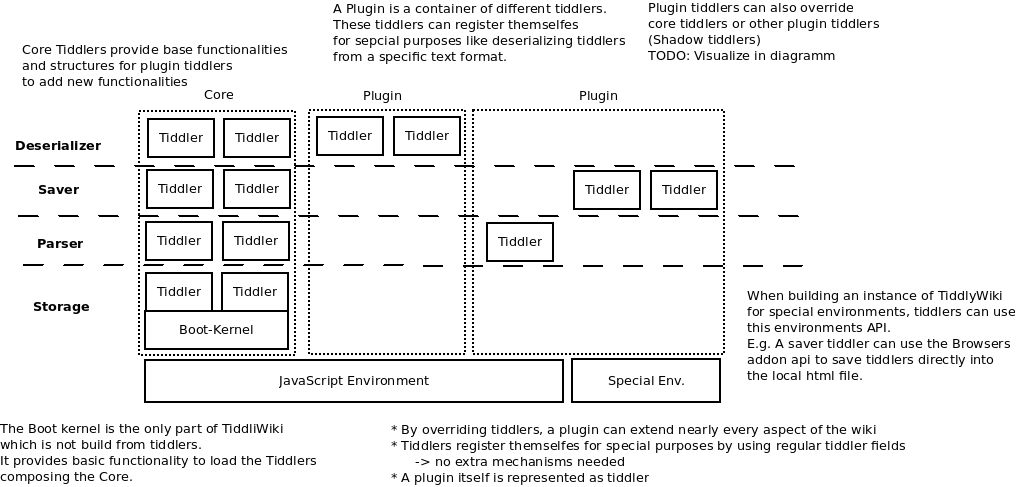
\includegraphics[scale=0.4]{images/overview.png}
\caption{Decomposition of TW}
\end{figure}
\newpage
\subsection{Tiddler as the key element 1}
A Tiddler is the smallest unit of the TiddlyWiki system. It can contains human readable text or other text-based content like javascript in the form of plugins. Internally Tiddlers are immutable objects contain a bunch of key:value pairs called fields. The only required field of a tiddler is the name field. For a list of the standard fields of a tiddler see (\prettyref{list:TiddlerFields})
\newpage
\subsection{The WikiText concept 1}
The WikiText is a markup language, created especially for the requirements of the TiddlyWiki application. It is based on Markdown\footnote{\url{http://daringfireball.net/projects/markdown/}}, but extended with some TiddlyWiki specific features.  On one hand its a text-to-HTML conversion language and on the other hand its used to provide the interactive features of TiddlyWiki. The aim of this language is to allow the user of the software to focus on the writing.\cite{TIDD:WIKITEXT} The WikiText is used to format Tiddlers within the TiddlyWiki application. The tags of the WikiText syntax can be used within the standard text input field. 
During the saving process these tags renders to HTML elements for example:
\begin{lstlisting}[caption={Example use of WikiText},label=lst:data-div]
WikiText:--- 
Renders as:
HTML:<hr>
WikiText:[img[http://tiddlywiki.com/favicon.ico]]
Renders as: 
HTML:<img src="http://tiddlywiki.com/favicon.ico">
\end{lstlisting}
Furthermore the WikiText is used to access the widgets which are integrated in the application.These widgets are used to enhance the the WikiText with a rich functionality. Widgets are based on the HTML-Syntax but always starts with a \$.
\begin{lstlisting}[caption={Example use of widgets within WikiText},label=lst:data-div]
WikiText:
<$button message="tw-close-tiddler">Close Me!</$button> 
\end{lstlisting}
\section{Bootstrap-Process 2-3}
\subsection{The Heart of TiddlyWiki (Boot-Kernel) 1 - 1.5}
\subsection{Timeline of the startup Process 1 - 1.5}

\section{The Plugin and Module concept 4-5}
\subsection{Introduction to the Plugin-Concept 1}
\subsection{Kernel-Plugins 1}
\subsection{UI-Elements 1}
\subsection{Developing a own Plugin 1-2}
\newpage
\section{The TiddlyWiki data management concept 2-3}
This section descripes how the data of the wiki is stored within Tiddlywiki during the runtime. And how the complete wiki is persistet.
\subsection{Data Management during Runtime 1-2}
During the runtime the data of Tiddlywiki is stored in javascript objects. These objects are synchronized with the DOM-Representation of Tiddlywiki. This means every change of the original data of a Tiddler, fires an event which changes all DOM-Representations of the Tiddler and the javascript object. The barbone Wiki store is created during the boot process and is kept in a object called \$tw.Wiki. This object contains amongst others a hashmap of the different Tiddlers of Tiddlywiki. The Hashmap is used to store the javascript object representation of the different Tiddlers.
\newpage 
\subsection{Data Persistence 1}
\subsubsection*{Persist data}
TiddlyWiki supports a wide range of methods to persist your data. One of this methods is the HTML5 fallback saver. This methods works on almost every browser. With this method a copy of the entire wiki will be downloaded by the browser. This means you get a new file everytime you hit the save button. To avoid this there a some plugins for different browsers to allow to save direct to the current open TiddlyWiki-File.
\subsubsection*{Data-Storage}
TiddlyWiki persists the data within the HTML-File in two Div-Areas depending on whether the encryption of the TiddlyWiki is activated or not. If the TiddlyWiki is not encrypted the data is stored in the Div-Area called ``StoreArea''. Every created Tiddler is stored in a own Div-area with a few custom values. An example of a saved Tiddler is shown below (\prettyref{lst:data-div}). 
\begin{lstlisting}[caption={Data-Div},label=lst:data-div]
<div created="20140611153703343" modified="20140611153734589" tags="testTag" testfield="testvalue" title="TestTiddler" type="text/plain">
	<pre>testText</pre>
</div>
\end{lstlisting}
The Div-Area has the following attributes, all attributes which are not in these list are parsed as a custom field:
\begin{description}
\label{list:TiddlerFields}
\item[created] Timestamp number of milliseconds since 01.01.1970.
\item[modified] Timestamp number of milliseconds since 01.01.1970.
\item[tags] list of tags seperated by whitespace. Tags which contain whitespaces are wrapped by [[ ]], e.g. [[example Tag]].
\item[type] Type of the Tiddler.
\item[title] Title of the Tiddler
\end{description}
With a activated encryption the data is stored in a special Div-Area called ``encryptedStoreArea''. TiddlyWiki uses the Standford JavaScript Crypto Libary\footnote{\url{http://bitwiseshiftleft.github.io/sjcl/}}. The encrypted Tiddlers are saved in a JSON string within this Div-Area.
\section{Summary and Conclusion 1-2}
\bibliography{tiddly}
\bibliographystyle{alpha}
\end{document}
